

The criterion we find is:
\par
There is a self-complementary graph on $n$ vertices if and only if $n=4k$ or $n=4k+1$ where $k \in \mathbb{N}$.
\begin{proof}
There are $n \choose 2$ edges in a complete graph of $n$ vertices, which means the sum of the edges of a graph and its complementary graph is $n \choose 2$.
$$|E|+|E'|={n \choose 2}$$
For a self-complementary graph, there is $|E| = |E'|$.
$$|E|=\frac{1}{2} {n \choose 2}=\frac{n(n-1)}{4}$$
Obviously, the edges of a graph should be an integer and as $n$ and $n-1$ must be one odd and one even, so 
$$n \equiv 0 \mod 4$$ 
or 
$$n-1 \equiv 0 \mod 4$$
these two conditions can be rewritten as
$$n=4k ~or~ 4k+1, \textbf{where} ~ k\in \mathbb{N}$$ 
Then we will prove the condition is sufficient by finding a self-complementary graph for $n=4k$ and $n=4k+1$.

\par
For $n=4k$, we split the vertices to $4$ groups with $k$ vertices in each group, as the following picture shows.

\begin{figure}[hpbt]
\begin{center}
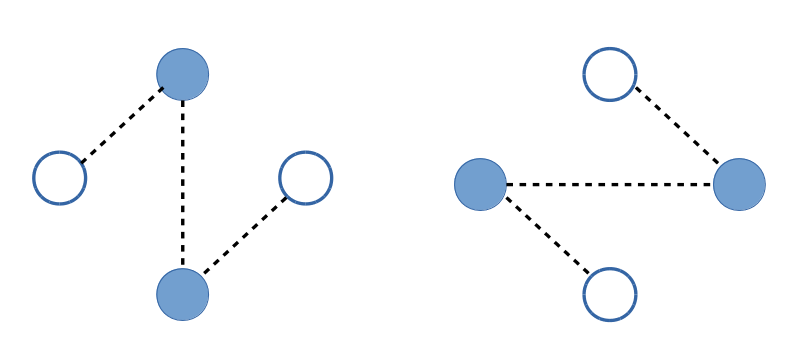
\includegraphics[width=0.6 \textwidth]{Ex6-6_1.png}
\end{center}
\end{figure}

A group in blue stands for the vertices in group is "fully connected", that is, $ \{u, v\} \in E $ for any two $u,v \in V_{blue}$. 
\par A group in white stands for there is no edge between any two vertices in white group. $ \{u, v\} \not \in E$ for any two $u,v \in V_{white}$.
\par The dot lines stands for there is an edge for any two vertices from groups the line connecting to. $ \{u, v\} \in E$ for $u \in V_1$, $v \in V_2$. 
\par 
The complementary graph of the left graph is the right graph. And we can easily see that they are isomorphic. So there is a self-complementary graph for $n=4k$.


For $n=4k+1$, we add one more vertex $x$ to the graph we found for $n=4k$.
\begin{figure}[hpbt]
\begin{center}
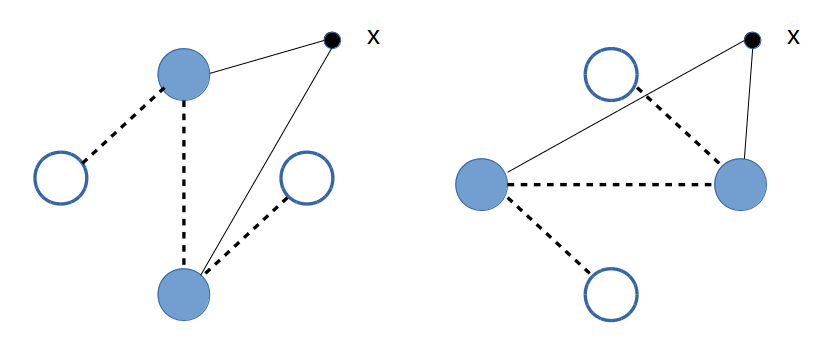
\includegraphics[width=0.6 \textwidth]{Ex6-6_2.png}
\end{center}
\end{figure}
Then we put edges between $x$ and vertices in blue groups. The black line stands for there is an edge between the vertex and any verterx in the group. $\{x, u\} \in E$ for any $u \in V_{blue}$.
\par
The graph's complementary graph is shown as well. We observe that they are isomorphic. So there is also a self-complementary graph for $n=4k+1$.   

\par So there is a self-complementary graph on $n$ vertices if and only if $n=4k$ or $n=4k+1$ where $k \in \mathbb{N}$.
\end{proof}